\phantomsection
\chapter{Motivations}

\noindent A facial expression is a "visible manifestation of the effective state, cognitive activity, intent, personality, and psychopathology of a person" \cite{DON99}; facial expressions represent a huge part in dialogue and interaction with other humans. Indeed, facial expressions carry more informations than speech, informations on which humans can relay for interaction. Facial expressions have a considerable effect on a listening interlocutor; in a conversation, it represents 55 percent of information received by a listener, while 38 percent are conveyed by voice intonation and the remaining 7 percent by the spoken words \cite{PAN00}.
\newline

\noindent Since Antiquity, researchers have been interested in emotion and more particularly in emotion recognition. One of the most important studies on facial expression analysis impacting on modern day science of automatic facial expression recognition is the work carried out by Charles Darwin \cite{BET12}. In 1872, Darwin wrote a book that established general expression principles, expression means and expression description for both humans and animals \cite{DAR04}. He also classified various kinds of expressions. This can be considered as the beginning of facial expression recognition.
\newline

\noindent Nowadays, with the emergence of new technologies and computers, research is now focused on computer-based automatic facial expression recognition. Because facial expressions are major factors in human interaction, this research field will improve the domain of Human-Machine Interaction. Indeed, emotion recognition will enable computers to be more responsive to users' emotions, and allow interactions to become more and more realistic. 
\newline

\noindent Another domain where facial expression recognition is an important issue is robotics. With the advances made in robotics, robots tend to mimic human emotion and react as as human-like as possible, especially for humanoid robots. Indeed, since robots are being more and more present in our daily lives, they need to understand and recognize human emotions.
\newline

<<<<<<< HEAD
\noindent A lot of applications in the robotics field have already emerged. For example, Bartlett et al. have successfully used their face expression recognition system to develop an animated character mirroring the expressions of the user (called CU Animate) \cite{BAR03}. They have also been successful in deploying the recognition system on Sony's Aibo Robot and ATR's RoboVie \cite{BAR03}. Another interesting application has been demonstrated by Anderson and McOwen, called "EmotiChat" \cite{AND06}. It is a regular chatroom, except the fact that their facial expression recognition system is connected to the chat and convert the users' facial expressions into emoticons. Because facial expression recognition systems' robustness and reliability are constantly increasing, lots of innovative applications will appear.
=======
\noindent A lot of applications in the robotics field have already been created. For example, Bartlett et al. have successfully used their face expression recognition system to develop an character that is animated and that mirrors the expressions of the user (called CU Animate) \cite{BAR03}. They have also been successful in deploying the recognition system on Sony's Aibo Robot and ATR's RoboVie \cite{BAR03}. Another interesting application has been demonstrated by Anderson and McOwen, called "EmotiChat" \cite{AND06}. It is a regular chatroom, except the fact that their facial expression recognition system is connected to the chat and convert the users' facial expressions into emoticons. Because facial expression recognition systems' robustness and reliability are constantly increasing, lots of innovative applications will appear.
>>>>>>> b610ac62028e14055893b066f33d934c6a720cdd
\newline

\noindent There are also various other domains where emotion recognition can be used: Telecommunications, behavioural science, video games, animations, psychiatry, automobile safety, affect-sensitive music jukeboxes and televisions, educational software, etc \cite{BET12}.
\newline

<<<<<<< HEAD
\noindent This project focuses on facial expression recognition from a video stream. Indeed, facial expression recognition can be performed \textit{statically} on input images, or \textit{dynamically} on video sequences. Systems can also be \textit{obtrusive}, or \textit{non-obtrusive}, the former based on a device mounted on the user's head or body, therefore following each of his movements and perform facial expression recognition without much losses, while the latter can encounter difficulties if the user is not properly situated. However, non-obtrusive systems allow more natural user interactions. We chose our system to be non-obtrusive, and will detail its setup further in the next section.
=======
\noindent This project focuses on facial expression recognition from a video stream. Indeed, facial expression recognition can be performed \textit{statically} on input images, or \textit{dynamically} on video sequences. Systems can also be \textit{obtrusive}, or \textit{non-obtrusive}, the former based on a device mounted on the user's head or body, therefore following each of his movements and perform facial expression recognition without much losses, while the latter can encounter difficulties if the user is not properly situated. However, non-obtrusive systems allow more natural user interactions. We chose our system to be non-obtrusive, and will detail further its setup in the next section.
>>>>>>> b610ac62028e14055893b066f33d934c6a720cdd
\newline

\phantomsection
\section{Environment Setup}

\vspace{\baselineskip}
\noindent Our system will use the camera embedded into a Microsoft Kinect to record the user's video input. We will consider a casual use of the camera, the user sitting in front of the computer, the camera being next to it, as seen in \textbf{\color{red} Insert picture of the setting \& ref to figure}. This camera provides a 640$\times$480 pixels frame resolution, while recording at 30 FPS.
\newline

\noindent For development and training purposes we will use some pre-existing emotion datasets, in order to validate the efficiency of the system before testing it in real conditions.
\newline

\phantomsection
\section{Facial Expression Datasets}

\vspace{\baselineskip}
\noindent Databases are very important for facial expression recognition system.
\newline

\noindent Using the same databases as in previous studies allows performance and accuracy comparisons between new implementations and previously obtained results. Since most studies draw their results on the same databases, it is then relatively easy to compare them and choose a database suitable for our system.
\newline

\noindent Databases are however difficult to build. Indeed, it has to be obtained following a meticulous procedure while being exhaustive so it can be considered as representative. The majority of actual databases use posed expressions rather than spontaneous ones, this choice having a major influence on facial expression recognition systems. This explains why some databases are updated, and now integrate spontaneous expressions. Even with this transition from posed expressions to spontaneous expressions, there are other requirements that should be met to have a standardized database.Its content should be of different resolutions and scales, and should also contain exposition under different conditions, i.e changes in lightning, occlusions or different head angles \cite{BET12}.  
\newline

\noindent Constructing a database is then a tedious task because of all these requirements to meet. Consequently, most studies are based on already existing datasets. The 3 datasets described afterwards are popular and freely available facial expression datasets which have been used a numerous amount of times in the past few years. Our system will then be trained and tested with one or several of these databases.
\newline

\subsection{Japanese Female Facial Expression Database (JAFFE)}

\vspace{\baselineskip}
\noindent This database contains 213 images of 7 facial expressions (6 basic facial expressions: happy, angry, afraid, disgusted, sad, surprised, and 1 neutral facial expression). Each expression has been photographed three or four times. Each image has been rated on 6 emotion adjectives by 60 Japanese subjects. All images come from 10 Japanese female models.  The database was planned and assembled by Miyuki Kamachi, Michael Lyons, and Jiro Gyoba \cite{JAFFE}.
\newline

\noindent This database contains only posed expressions. The photos have been taken under strict  and controlled conditions: similar lighting and hair tied so there is no facial occlusion \cite{BET12}. 
\newline

\noindent An example of images contained in the database is given by Figure~\ref{jaffe_7facialexpressions}. In this figure, this is a female subject displaying 7 different emotional expressions (neutral, happy, angry, afraid, disgusted, sad, surprised). 
\newline

\begin{figure}[!h]
\begin{center}
\noindent 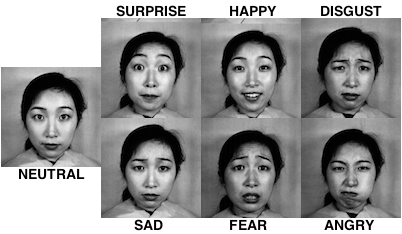
\includegraphics[scale=0.75]{figures/jaffe_7facialexpressions} 
\newline
\caption{Example of images from JAFFE database}
\label{jaffe_7facialexpressions}
\end{center} 
\end{figure}

\subsection{Karolinska Directed Emotional Faces Database (KDEF)}

\vspace{\baselineskip}
\noindent The Karolinska Directed Emotional Faces (KDEF) contains 4900 pictures of human facial expressions. The material was developed in 1998 by Daniel Lundqvist, Anders Flykt and Professor Arne Ohman at Karolinska Institutet, Department of Clinical Neuroscience, Section of Psychology, Stockholm, Sweden \cite{KDEF}.
\newline

\noindent The database was first developed for psychological and medical research purposes. It was created so it could used in perception, attention, emotion, memory and backward masking experiments. This database has also been built under controlled conditions. Indeed, researchers tried to maintain constant and soft lighting for each subject. Furthermore, they made their subjects wear the same grey T-shirts, and used a grid to center the participants faces while they were shot. This grid was also used to place eyes and mouths at the same position in fixed image coordinates during scanning \cite{KDEF}.
\newline

\noindent The database contains 70 individuals (35 males and 35 females), from 20 to 30 years, each one displaying 7 different emotional expressions (neutral, happy, angry, afraid, disgusted, sad, surprised). Each expression has been photographed (twice) from 5 different angles (-90, -45, 0, +45, +90 degrees: i.e. full left profile, half left profile, straight, half right profile, full right profile)  \cite{KDEF}.
\newline

\noindent An example of images contained in the database is given in Figure~\ref{kdef_7facialexpressions}which represents a female subject photographed from a straight angle and displaying 7 different emotional expressions (neutral, happy, angry, afraid, disgusted, sad, surprised).
\newline

\begin{figure}[!h]
\begin{center}
\noindent 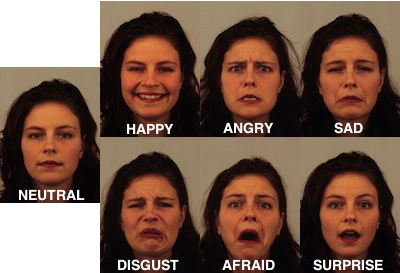
\includegraphics[scale=0.65]{figures/kdef_7facialexpressions} 
\newline
\caption{Example of images from KDEF database}
\label{kdef_7facialexpressions}
\end{center} 
\end{figure}

\subsection{Montreal Set of Facial Displays of Emotion Database (MSFDE)}

\vspace{\baselineskip}
<<<<<<< HEAD
\noindent This database contains facial expressions of European, Asian, and African subjects, from both genders. Each expression was created by directly asking the subject to express this emotion \cite{MSFDE}.
=======
\noindent The database contains facial expressions of men and women from European, Asian, and African type. Each expression was created by asking directly the subject to express this emotion and all expressions were FACS coded in order to assure identical expressions among the subjects \cite{MSFDE}.
>>>>>>> b610ac62028e14055893b066f33d934c6a720cdd
\newline

\noindent The database contains expressions of happiness, sadness, anger, fear, disgust, and embarrassment, along with a neutral facial expression. All expressions have been photographed at 5 different levels of intensity \cite{MSFDE}.
\newline

\noindent An example of images contained in the database is given in Figure~\ref{msfde_7facialexpressions}, where an African female subject displays 7 different emotional expressions (neutral, happy, angry, afraid, disgusted, sad, ashamed).
\newline

\begin{figure}[!h]
\begin{center}
\noindent 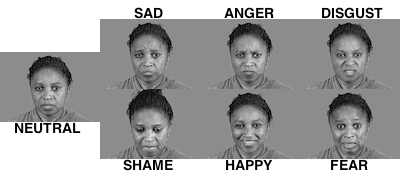
\includegraphics[scale=0.8]{figures/msfde_7facialexpressions} 
\newline
\caption{Example of images from MSDFE database}
\label{msfde_7facialexpressions}
\end{center} 
\end{figure}






